
\subsection{Mutanty i mutacje}
\index{mutant|(}%
\index{mutacja|see {mutant}}%
\label{sec:mutant}%
Na zakończenie wspomnimy o~mutacjach.

\begin{definition}[mutacja]
    % \labelnotinuse{def:mutacja}
    Półobrót supła względem osi poziomej, pionowej albo też prostopadłej do płaszczyzny, w~jakiej leży diagram, nazywamy mutacją.
    W razie potrzeby zmieniamy orientację supła na przeciwną.
\end{definition}

\begin{definition}[mutant]
\label{def:mutant}%
    Niech $K$ będzie węzłem.
    Węzeł, który powstaje przez wykonanie ciągu mutacji na węźle $K$, nazywamy mutantem węzła $K$.
\end{definition}

Mutacja węzła o~co najwyżej dziesięciu skrzyżowaniach nie zmienia jego klasy abstrakcji.
Najprostszą, a zarazem najsłynniejszą parą różnych od siebie mutantów stanowią węzeł Conwaya $11n_{34}$ oraz Kinoshity-Terasakiego $11n_{42}$.
\index{węzeł!Conwaya}%
\index{węzeł!Kinoshity-Terasakiego}%

\begin{figure}[H]
\centering
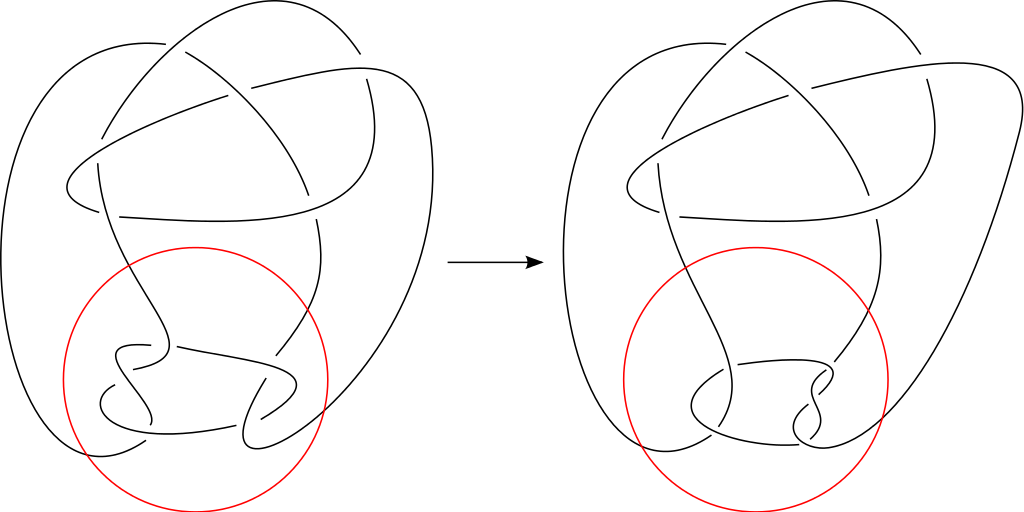
\includegraphics[width=0.601\linewidth]{../data/mixed/knudemutation.png}
\caption{Węzły $11n_{42}$ oraz $11n_{34}$. Grafika Sørena Jørgensena, dostępna na licencji \href{https://creativecommons.org/licenses/by-sa/3.0/deed.en}{CC BY-SA 3.0} pod adresem \url{https://en.wikipedia.org/wiki/File:Knudemutation.svg}.}
\end{figure}
Conway zauważył podczas klasyfikacji niealternujących węzłów, że tylko one posiadają trywialny wielomian Alexandera.
Mają też taki sam wielomian Jonesa,
\begin{equation}
    \jones(t) = t^{6} -2t^5 +2t^4 -2t^3 +t^2 +2t^{-1} -2t^{-2} +2t^{-3} -t^{-4}.
\end{equation}
Kinoshita, Terasaki zdefiniowali nieskończoną rodzinę węzłów o trywialnym wielomianie Alexandera, której pierwszym wyrazem jest węzeł $11n_{42}$ w~\cite{kinoshita57}.
\index[persons]{Kinoshita, Shinichi}%
\index[persons]{Terasaka, Hidetaka}%
Dowód tego, że $11n_{34}$ oraz $11n_{42}$ są różne, jako pierwszy podał prawdopodobnie Riley w~1971 roku \cite{riley71}: wykorzystał on homomorfizmy z~grupy węzła w~$PSL(2, 7)$.
\index[persons]{Riler, ?}%
%=% "The inequivalence of these knots was first observed by [Riley 1971]." - Kawauchi, strona 44
Genusy, odpowiednio: $3$ i~$2$, wyznaczył Gabai piętnaście lat później w~\cite{gabai86}, używał foliacji.
\index[persons]{Gabai, David}%

Niedawno Stojmenow podjął się systematycznie szukania mutantów wśród węzłów o~mniej niż 19 skrzyżowaniach (praca \cite{stoimenow10} z~2010 roku).
\index[persons]{Stoimenow, Alexander}%
Początkowo pracował sam, badając pewne subtelne przykłady postanowił uwikłać w swój projekt Toshifumiego Tanakę, a później także Daniela Mateię.
\index[persons]{Tanaka, Toshifumi}%
\index[persons]{Daniel, Matei}%
Praca \cite{stoimenow10} jest kontynuacją artykułu, który napisali wspólnymi siłami.

I tak na stronie 531 można przeczytać, że ,,niezmienniki Wasiljewa co najwyżej 8. stopnia nie rozróżniają mutantów węzłów \cite{chmutov94}'', ja tego nie widzę.
\index{niezmiennik!Wasiljewa}%
Mniej więcej sześć lat później wynik poprawił J. Murakami (nie mylić z H. Murakamim!) do 10. stopnia w~niezindeksowanej pracy \cite{murakami99}.
\index[persons]{Murakami, Jun}
W międzyczasie Cromwell, Morton znaleźli niezmiennik stopnia 11., który odróżnia węzły Conwaya oraz Kinoshity-Terasakiego; patrz \cite{cromwell96}.
\index[persons]{Cromwell, ?}%
\index[persons]{Morton, Hugh}%
% czy Murakami potwierdził wynik Cromwella, Mortona?

Mutant węzła złożonego także jest złożony, co więcej istnieje bijekcja między czynnikami w ich rozkładach na węzły pierwsze Ruberman -- \cite{ruberman87}.
\index[persons]{Ruberman, Daniel}%
Dzięki temu możemy bez straty ogólności założyć, że badamy tylko węzły pierwsze, niestety wciąż nie jest znana ogólna procedura pozwalająca wyliczyć wszystkie mutanty danego węzła.

Zaraz po rewolucji, jaką w latach 80. wywołała relacja kłębiasta, Ewing napisał z~Millettem komputerowy program w~języku C, który wyjątkowo szybko znajdował wielomiany HOMFLY oraz Kauffmana zadanego węzła.
\index[persons]{Ewing, ?}%
\index[persons]{Millett, Kenneth}%
Nawet dziś program ten jest w stanie uporać się z węzłami, z którymi nie radzą sobie inne narzędzia.
Autorzy nie wiedzieli wtedy, że ktoś jeszcze będzie z nich korzystać w przyszłości, dlatego poczynili w kodzie liczne optymalizacje dla stacji roboczej Sun, jaką wtedy dysponowali.
Dzisiaj okazuje się, że dla węzłów o większej liczbie skrzyżowań program często kończy swoje działanie zrzutem pamięci, wpada w pętlę bez wyjścia albo zwraca niepoprawny wynik (składniki wielomianu Kauffmana są postaci $a^m z^n$, gdzie $m + n$ jest nieparzyste).
Stojmenow korzystał z tych programów podczas tablicowania mutantów.
Jak postępował?
\begin{enumerate}
    \item podzielił węzły na grupy o tej samej objętości, wielomianie Jonesa oraz Alexandera;
    \item w każdej z grup szukał ciągu mutacji pomiędzy diagramami minimalnymi;
    \item tam, gdzie nie udało się znaleźć mutantów, liczył 2-kablowy wielomian HOMFLY;
    \item jeśli wielomian był taki sam, szukał ciągu mutacji między nieminimalnymi diagramami do 18 skrzyżowań;
    \item wreszcie pozostałe grupy zostały potraktowane reprezentacjami grupy podstawowej dwukrotnego nakrycia.
\end{enumerate}

Podsumowanie jego pracy zawiera tabela:

\begin{table}[H]
    \centering
    \begin{tabular}{lccccc} \toprule
        skrzyżowania & 11 & 12 & 13  & 14   & 15    \\ \midrule
        pary         & 16 & 70 & 703 & 3917 & 24884 \\
        trójki       &    & 5  & 38  & 233  & 1000  \\
        czwórki      &    &    & 32  & 262  & 2909  \\
        szóstki      &    &    & 1   & 17   & 172   \\
        ósemki       &    &    &     & 6    & 84    \\
        łącznie      & 16 & 75 & 774 & 4435 & 29049 \\
        \bottomrule
        \hline
    \end{tabular}
    \caption{Liczba grup mutantów wśród pierwszych węzłów do 15 skrzyżowań}
\end{table}

\subsubsection{Rozróżnianie mutantów}
Żaden wielomianowy niezmiennik opisany w~tej książce nie potrafi odróżnić od siebie węzłów $11n_{34}$ oraz $11n_{42}$.
Okazuje się, że niewielomianowe niezmienniki też często są bezradne.

\begin{proposition}
    Mutacja węzła nie zmienia jego wielomianu Alexandera.
\index{wielomian!Alexandera}%
\end{proposition}

% w commicie 1fe48ad183cb592e897f4151f9c18439baa84274 wymieniam:
% +    kablowego wielomianu Jonesa, % menasco91
% +    2-kablowego wielomianu HOMFLY, % przytycki89
% +    kablowego wielomianu Kauffmana, % lipson87
% +    sygnatury Tristrama-Levine'a, % cooper99
% +    symplicjalnEj objętości Gromowa, % ruberman87
% +    instanton homologii Floera, % ruberman99
% +    niezmienników Wittena % rong94
% +    ani Cassona. % kirk89
% ale teraz nie potrafię sobie przypomnieć, jak znalazłem te niezmienniki/prace. :(
% wydaje mi się, że źródłem nie jest stoimenow10, może Math Overflow?

\begin{proof}
    Stojmenow, Tanaka piszą w \cite{tanaka09}, że to proste ćwiczenie teorii kłębiastej, oraz że rozumowanie łatwo przenosi się na odkryte później wielomiany Jonesa, HOMFLY, BLM/Ho, Kauffmana.
\end{proof}

Warto przytoczyć teraz obserwację 3.8.2 z \cite[s. 43]{kawauchi96}: jeśli sploty $L_1, L_2$ są mutantami, to podwójne przestrzenie nakryciowe nad $S^3$ rozgałęzione odpowiednio wzdłuż $L_1$ oraz $L_2$ są homeomorficzne z zachowaniem orientacji.
Co więcej, macierze Seiferta mutantów są $S$-równoważne.
\index{macierz!Seiferta}%
To tłumaczy czemu większość niezmienników nie radzi sobie z odróżnianiem mutantów.
% Viro: Two-fold branched coverings of three-sphere

% z tanaka09
Wzór kablowy\footnote{Niech $T$ będzie trywialnym torusem, zawierającym węzeł $K$, zaś $e \colon T \to S^3$ włożeniem $T$ na otoczenie węzła $C$ tak, że $e$ przenosi równoleżnik $T$ na równoleżnik $C$. Wtedy $\alexander_{eK} (t) = \alexander_K(t)\alexander_C(t^n)$.} \cite[tw. 6.15]{lickorish97} pokazuje, że wielomian Alexandera nie odróżnia satelitów zmutowanych węzłów.
Wielomian Jonesa nie spełnia żadnego wzoru kablowego (gdyż czasami odróżnia kable węzłów o~tym samym wielomianie), ale...:

\begin{proposition}
    Mutacja węzła nie zmienia jego kablowego wielomianu Jonesa.
\index{wielomian!Jonesa}%
\end{proposition}

\begin{proof}
\index[persons]{Morton, Hugh}%
\index[persons]{Traczyk, Paweł}%
    Morton, Traczyk \cite{traczyk88}.
    % kiedyś tu było niezdefiniowane menasco91 = Menasco, Thistlethwaite: The Tait flyping conjecture, ale w 2022 roku przeczytałem Stoimenow: Tabulating and distinguishing mutants zmieniłem zdanie: "nonetheless Morton and Traczyk [36] showed that..."
\end{proof}

Praca \cite{traczyk88} wspomina jeszcze, że to samo jest prawdą także dla ,,wielomianu Jonesa dwóch zmiennych'' (HOMFLY) i 2-kabli, ale nie dla dowolnych satelitów.
Fakt, że wielomian HOMFLY (a także Kauffmana) nie odróżniają 2-satelitów mutantów, odkryto rok wcześniej:

\begin{proposition}
\label{mutants_and_homfly}%
\index{wielomian!HOMFLY}%
    Mutacja węzła nie zmienia jego 2-kablowego wielomianu HOMFLY.
\end{proposition}

\begin{proof}
\index[persons]{Lickorish, William}%
\index[persons]{Lipson, ?}%
\index[persons]{Przytycki, Józef}%
    Lickorish, Lipson \cite{lipson87}, później też Przytycki \cite{przytycki89}.
    % TODO: skąd to o Przytyckim???
\end{proof}

Lepiej jest z~3-kablami: wielomian HOMFLY odróżnia tak węzły Kinoshity-Terasakiego i~Conwaya, ale wymaga takiej ilości rachunków, że mało komu chce się je przeprowadzać dla innych węzłów.
\index{węzeł!Conwaya}%
\index{węzeł!Kinoshity-Terasakiego}%

\begin{proposition}
    Mutacja węzła nie zmienia jego (2-?)kablowego wielomianu Kauffmana.
\index{wielomian!kablowy}%
\index{wielomian!Kauffmana}%
\end{proposition}

\begin{proof}
\index[persons]{Lickorish, William}%
\index[persons]{Lipson, ?}%
    Lickorish, Lipson \cite{lipson87}.
\end{proof}

Morton w recenzji pracy Lickorisha, Lipsona wspomina, że dla satelitów owijających się więcej niż $2$ razy to nie jest prawda, jak później odkryto.

\begin{proposition}
\index{wielomian!BLM/Ho}%
    Mutacja węzła nie zmienia jego wielomianu BLM/Ho.
\end{proposition}

\begin{proof}
    \cite{tanaka09}, choć nie wiem gdzie dokładnie.
\end{proof}

\begin{proposition}
\index{sygnatura!Levine'a-Tristrama}%
    Mutacja węzła nie zmienia jego sygnatury Levine'a-Tristrama.
\end{proposition}

\begin{proof}
\index[persons]{Cooper, ?}%
\index[persons]{Lickorish, William}%
    Cooper, Lickorish w~\cite{cooper99} podają klasyczny dowód, że mutacja zachowuje wielomian Alexandera, oparty o~macierz Seiferta.
    Wiedząc, jak wygląda ta macierz, autorzy wyciągają wniosek, że sygnatura splotów (!) w~homologicznej 3-sferze też jest zachowywana.
\end{proof}

\begin{proposition}
\index{objętość!symplicjalna Gromowa}%
\label{mutants_the_same_volume}%
    Mutacja węzła nie zmienia jego symplicjalnej objętości Gromowa.
\end{proposition}

\begin{proof}
\index[persons]{Ruberman, Daniel}%
    Ruberman w \cite{ruberman87}.
    % Ruberman [42] showed that mutants have equal volume in all hyperbolic pieces of the JSJ decomposition.
\end{proof}

\begin{proposition}
\index{homologia!Floera}%
    Mutacja węzła nie zmienia jego instanton homologii Floera.
\end{proposition}

\begin{proof}
\index[persons]{Ruberman, Daniel}%
    Jeszcze raz Ruberman, w \cite{ruberman99}.
\end{proof}

\begin{proposition}
\index{niezmiennik!Wittena}%
    Mutacja węzła nie zmienia jego niezmienników Wittena.
\end{proposition}

\begin{proof}[Niedowód]
    Rong dla wybranych mutacji (niech $L$ będzie obramowanym splotem w~3-rozmaitości $M$, zaś $F \subseteq M$ dwustronną powierzchnią, tnącą splot w 0, 1 lub 4 (transwersalnie) punktach, o genusie $g = 0$, $1$ lub $2$, wtedy rozcięcie $M$ wzdłuż $F$ i sklejenie po obrocie o 180 stopni daje parę $(M^\tau, K^\tau)$, która ma ten sam niezmiennik Wittena w $\mathrm{SU}(2)$ jak wyjściowa) w \cite{rong94}.
\end{proof}

\begin{proposition}
\index{niezmiennik!Cassona}%
    Mutacja węzła nie zmienia jego niezmienników Cassona.
\end{proposition}

Celowo nie podajemy definicji tego niezmiennika.
Nieformalnie, zlicza on co drugą klasę sprzężoności reprezentacji grupy podstawowej homologicznej 3-sfery w grupie $SU(2)$.

\begin{proof}
    Kirk w \cite{kirk89}.
\end{proof}

\begin{conjecture}
    Mutacja węzła nie zmienia jego liczby gordyjskiej.
\end{conjecture}

Jak czytamy w \cite[problem 1.69]{kirby78}, przypuszczenie to jest bardzo trudne do udowodnienia: wynika z niego inna stara hipoteza teorii węzłów, że liczba gordyjska splotów jest addytywna.
\index{hipoteza!o indeksie skrzyżowaniowym}%
Przytoczymy tylko dwa częściowe wyniki.
Najpierw Rolfsen zauważył, że jedynym mutantem niewęzła jest sam niewęzeł \cite{rolfsen93}.
\index[persons]{Rolfsen, Dale}%
Dekadę później Gordon, Luecke pokazali, iż klasa węzłów $1$-gordyjskich jest zamknięta na przeprowadzanie mutacji \cite{gordon06}.
\index[persons]{Gordon, Cameron}%
\index[persons]{Luecke, ?}%
(Ohtsuki powtarza hipotezę w \cite[problem 12.15]{ohtsuki02}.)
\index[persons]{Ohtsuki, ?}%

% to NIE jest z stoimenow10
\begin{proposition}
    Niech $D$ będzie alternującym diagramem.
    Wtedy każdy mutant $D$ też jest alternujący.
\end{proposition}

Wśród niezmienników, które mutacja czasami zmienia, znajduje się genus plastrowy:

\begin{proposition}
\index{genus!plastrowy}%
    Niech $m, n$ będą nieujemnymi liczbami całkowitymi.
    Wtedy istnieje węzeł $K$ o genusie plastrowym równym $m$, którego pewien mutant ma genus plastrowy równy $n$.
\end{proposition}

Stanowi to uogólnienie obserwacji Livingstona \cite{livingston83}, że istnieją mutanty o~różnym genusie plastrowym.
\index[persons]{Livingston, Charles}%

\begin{proof}
    Kim, Livingston w \cite{kim05}.
\end{proof}

Zbiór problemów niskowymiarowej topologii opublikowany przez Kirby'ego \cite{kirby78} zawiera następujące pytanie:
\index[persons]{Kirby, Rob}%

\begin{conjecture}[problem 1.91]
\index{węzeł!satelitarny}
    Niech $K$ będzie prostym\footnote{simple} węzłem bez orientacji.
    Czy istnieją węzły niebędące mutantami $K$, których nie można odróżnić od $K$ wielomianem Jonesa oraz wszystkimi jego satelitami?
\end{conjecture}

Stojmenow pisze, że tak: pierwszą chronologicznie parą jest $14_{41721}$, $14_{42125}$, dowód tego faktu opiera się na wzorze fuzyjnym Masbauma-Vogela odkrytym w pracy \cite{masbaum94}.
\index[persons]{Stoimenow, Alexander}
\index[persons]{Masbaum, Gregor}%
\index[persons]{Vogel, Pierre}%
% fusion formula
Choć wzór ten zastosowany do konkretnej pary węzłów sprawia zazwyczaj trudności rachunkowe, to jest wystarczającym narzędziem, by rozszerzyć konstrukcję do ogólnego wyniku:

\begin{proposition}
    Istnieje nieskończenie wiele par prostych węzłów hiperbolicznych o tych samych kolorowych wielomianach Jonesa, które nie są swoimi mutantami.
\end{proposition}

\begin{proof}
    Stojmenow, Tanaka \cite[tw. 1.1]{tanaka09}.
\end{proof}

\index{mutant|)}

